\documentclass[11pt]{article}
\usepackage{graphicx}
\usepackage{amssymb}
\usepackage{amsthm, amsmath}
\usepackage{fancyhdr}


\usepackage{biblatex}
\usepackage[colorlinks,citecolor=green,urlcolor=blue,bookmarks=false,hypertexnames=true]{hyperref} 
\newtheorem*{theorem}{Theorem}
\newtheorem{lemma}{Lemma}
\newtheorem{proposition}{Proposition}
\newtheorem*{corollary}{Corollary}

\newcommand{\ABox}{
\raisebox{3pt}{\framebox[6pt]{\rule{6pt}{0pt}}}
}
%\newenvironment{proof}{{\bf Proof:}}{\qquad\ABox}
%-------------------------------------------------
\newtheorem{observation}{Observation}
\newtheorem{definition}{Definition}
\newtheorem{conjecture}{Conjecture}

\usepackage[boxed]{algorithm}
\usepackage[noend]{algorithmic}
\usepackage{wrapfig}
\usepackage[algo2e,linesnumbered]{algorithm2e}
\usepackage{csquotes}

\setlength{\topmargin}{0pt}
\setlength{\textheight}{9in}
\setlength{\headheight}{15pt}
\setlength{\headsep}{25pt}
\setlength{\oddsidemargin}{0.25in}
\setlength{\textwidth}{6in}



\begin{document}

\thispagestyle{empty}

\begin{titlepage}
    \begin{center}
        \vspace*{1cm}
        \Huge
        \textbf{CS6400 - Individual Project Proposal\\}
        \vspace{0.8cm}
        \Large
        Chen, Te-Kai MS-CSE\\
        email: tchen483@gatech.edu\\
             
    \end{center}
 \end{titlepage}
%%%%%%%%%%%%%%%%%%%%%%%%%%%%%%%%%%%%%%%%%%%%%%%%%%%%%%%%%%%%%%%%
%% BODY OF SCRIBE NOTES GOES HERE
%%%%%%%%%%%%%%%%%%%%%%%%%%%%%%%%%%%%%%%%%%%%%%%%%%%%%%%%%%%%%%%%
\pagestyle{fancy}
\fancyhf{}
\rhead{tchen483@gatech.edu}
\lhead{Chen, Te-Kai MS CSE}
\rfoot{Page \thepage}

\section{ERR Model}

\begin{figure}[h!]
    \centering
    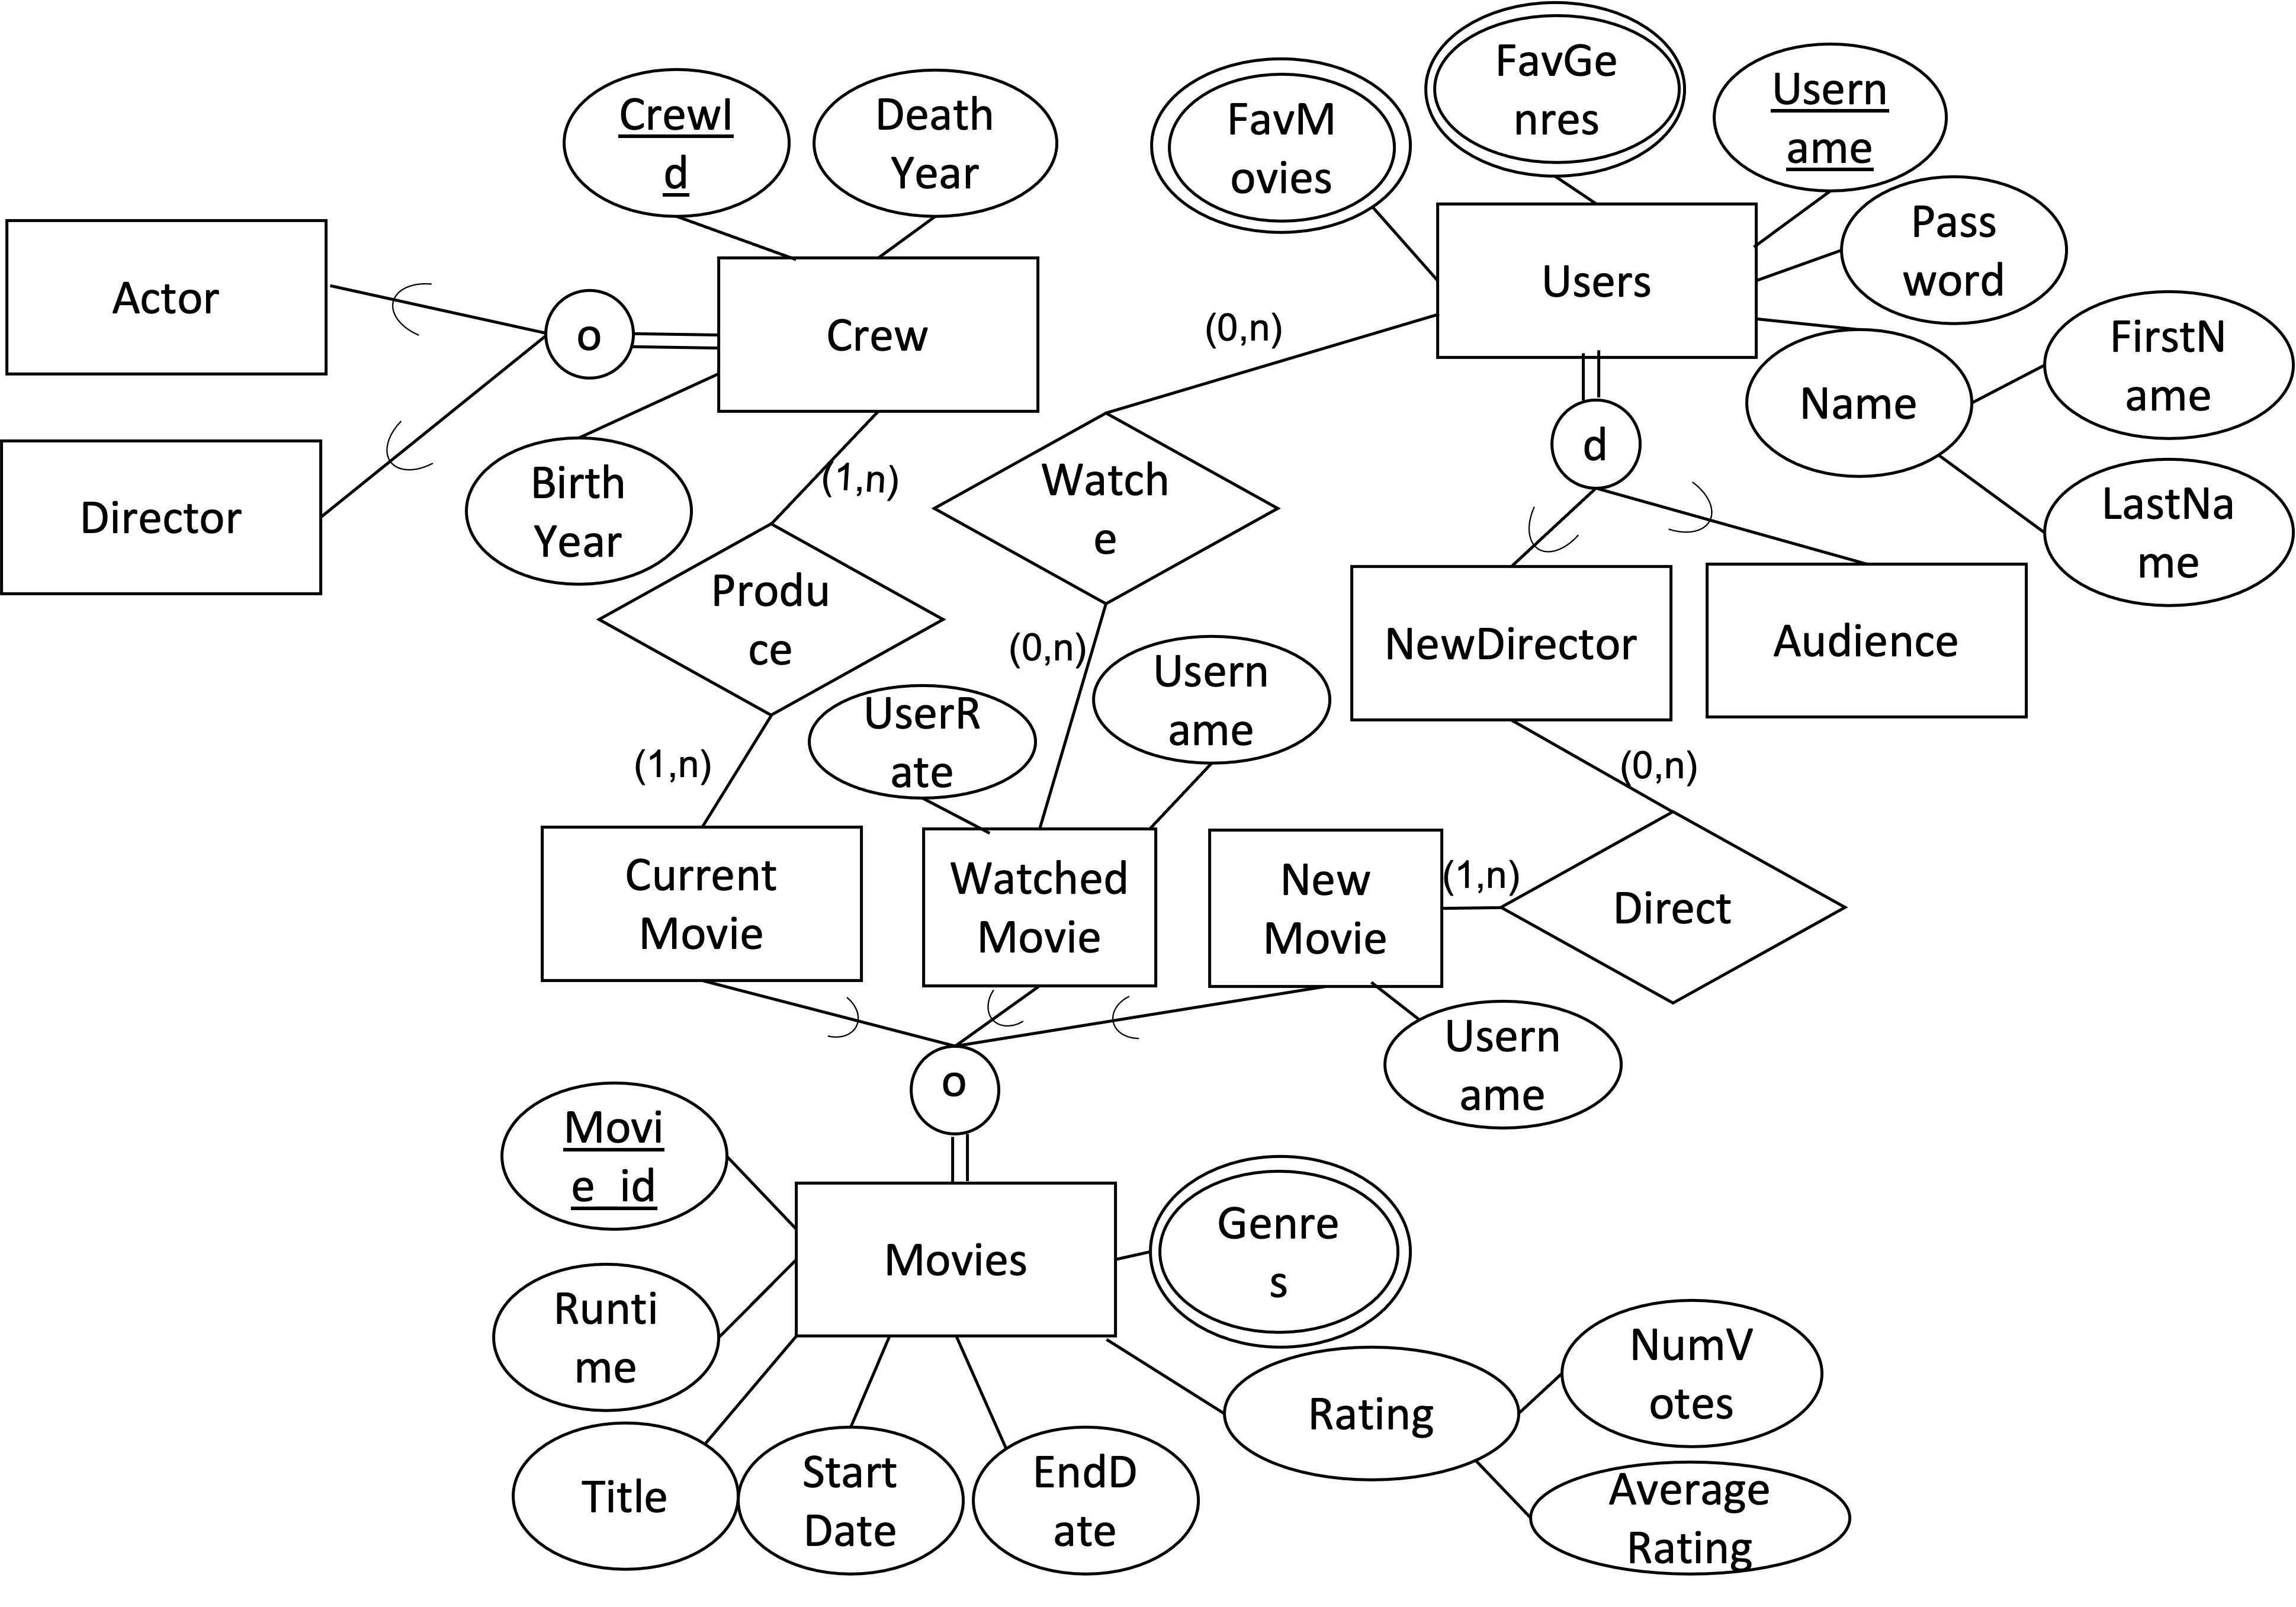
\includegraphics[scale=0.5]{Revised_EER.png}
    \label{fig:ER_Model}
\end{figure}
\section{Application}

Design a website based on an IMDB movie dataset 
which can let users search the top-rated movies with user's preference 
There are two types of users, one is the normal users, the other is directors. All users can use the search function, for example, find out what the movies and TV series ratings are and other searching usages. \\
For normal audiences, they can add their favorite movie, actor, director, and genre to their list. and the web will recommend some high rating movies or some TV series having high related to their favorite movies.\\
For directors and writers, they can add the newest movies that they have produced. Also, the system will list some movies which are related to the director's movies and tell the user these movies may become its competitor.
\section{Functionality}
There will be multiple functions and queries about searching the movies including basic search options. 
For instance, We can set the minimum rating of the movie or search the movie with specific 
directors/writers. \\
\begin{enumerate}
    \item \textbf{Registration}: Allow users to create accounts. Creating new account will need to fill in the username and password 
    and require them to fill their first name, second name, email, birthdate and whether they are directors or not. 
    Furthermore, the new users should at least specify 3 genres or movies to 
    help the recommendation works. The username should be unique for each user.\\
    \item \textbf{Login}: Users can use the username and password to login to access their personal favorite movies.\\
    \item \textbf{Rating movies}: Users can rate the movies and set their favorite genres.\\
    \item \textbf{Movie Recomemndation}: After Users login into their account, the website will randomly 
    recommends the fittest movies for them depending on genres and movies they have already seen and the information of the users \\
    \item \textbf{For director-only}: Add new movie into database.
\end{enumerate}
\textbf{For all users - Query}
\begin{itemize}
    \item Search the highest rate movies \\
    \item Search the movies with specific $startDate$ \\
    \item Search the movies with specific $endDate$ \\
    \item Search the movies with specific $genre$ \\
    \item Search the movies with specific $actors$  \\
    \item Search the movies with specific $director$ \\
    
\end{itemize}
The website will also calculate the average rating of actors and directors depending on the movies they have produced. As I mentioned above, there are some utilities for directors and normal users, and these will be implemented into my project too.

\section{Data, DBMS, Language}
Data: IMDB movie dataset, I get it from https://www.imdb.com/interfaces/. 
I'm going to use five tsv data on the website.\\ 
DMBS: MySQL\\ 
Language: HTML + CSS + php

\section{Interface Design}
The website will have two pages, landing page, and the searching/result page
On the landing page, users have to log in or create a new account for accessing the website.
After logging into their account, then the user can start accessing the database through the search bar. There may have some random recommendation of 
movie/ TV series on the top or bottom in the landing page also.

\section{Scope}
I'll implement the functionality that I have mentioned above, 
including the basic search function and some advanced search options. Also, 
the authority of accessing specific utility between normal users and directors 
will be decided using the login data. There are some additional features that I want to implement. 
One is adding the movie trailer and introduction to each movie and TV series. 
Another is to connect to the IMDB website to update the database weekly since there will be new 
films and ratings every week.


% \\
% We now analyze $f(x) = 1 - (1 - q \cdot x)^d$ and will get Eq~\ref{eq3} by differentiate Eq~\ref{eq2}
% If we let $x = 0$, then we can get Eq~\ref{eq4}, indicating that $f'(x)$ is monotone decreasing between [0,1]
 
% \begin{align}
%     \label{eq3} % Equation label; can be used for referencing
%     f(x) = q \cdot(1 - qx)^{d - 1}
% \end{align}
% \begin{align}
%     \label{eq4} % Equation label; can be used for referencing
%     f'(0) = q \cdot d
% \end{align}
% \begin{figure}[h!]
%     \centering
%     \includegraphics[scale=0.3]{FixP2.png}
%     \caption{Expecting f(x) for pandemic to die out}
%     \label{fig:FP2}
% \end{figure}
% Hence, we need to let Eq~\ref{eq4} $< 1$ so $f(x)$ can be below $y = x$, like Figure~\ref{fig:FP2},
% In this scenario, the pandemic can finally disappear. In this paragraph,
% we find out that $q \cdot d$ should $< 1$, and $q \cdot d$ is the expected number
% of people we infect. This is the same as the Reproductive number $R_0$ in ODE.
% In conclusion, this model also has the same idea of the ODE mentioned in previous lecture.
% However, this random tree model can only describe the begining of the pandemic 
% since each node can only meet d people once, which is impossible in reality.



% \subsection{General Graph}

% \subsubsection{SIR model}
% In SIR model, each node in the graph Figure~\ref{fig:GraphSIR} is a person and always represent one of the 
% three states. There are Susceptible(Marked with white), Infected(Marked with yellow), 
% Recovered(Marked with sheild). 
% \\
% \begin{figure}[h!]
%     \centering
%     \includegraphics[scale=0.5]{GraphSIR.png}
%     \caption{Exapmle of Graph SIR model}
%     \label{fig:GraphSIR}
% \end{figure}

% When $t = 1$, we find out that there is one infected in the Node and it has the probability of $\beta$ 
% to infect other nodes which are connected to it and has the probability of $\delta$ to cure itself. 
% In other words, when t change, the infected node will have $\beta$ probability to mark its neighbors 
% yellow and $\delta$ to mark itself become shield.\\
% In Figure~\ref{fig:Initial_SIR} to Figure~\ref{fig:500Itr}, we show some simulation of the SIR model with one infected node marked with green. The blue node is susceptible, 
% red one is infected and the gray one is recovered.
% \begin{figure}[h!]
%     \centering
%     \includegraphics[scale=0.5]{Initial_SIR.png}
%     \caption{Initial SIR graph model with one infected node}
%     \label{fig:Initial_SIR}
% \end{figure}
% \begin{figure}[h!]
%     \centering
%     \includegraphics[scale=0.4]{200_400_Itr.png}
%     \caption{Left: 200 Iteration, Right: 400 Iteration}
%     \label{fig:200_400_Itr}
% \end{figure}
% \begin{figure}[h!]
%     \centering
%     \includegraphics[scale=0.4]{500Itr.png}
%     \caption{Left: 500 Iteration, Right: End of pendemic}
%     \label{fig:500Itr}
% \end{figure}
% \newpage
% Figure~\ref{fig:SIR_London} is a diagram from the website \url{http://epirecip.es/epicookbook/chapters/london-boroughs-network/r}, 
% We can see that this diagram is similar to the ODE diagram before.
% However, we can see that the curve of I(green one) sometimes go up and down, which is different 
% from the ODE diagram. It is because each node in network model may have different degree so the 
% I curve is not stable. That's also why we prefer to use the network to describe pandemic since 
% its result is more close to reality.
% \begin{figure}[h!]
%     \centering
%     \includegraphics[scale=0.45]{SIR_London.png}
%     \caption{London's time-value diagram of SIR model}
%     \label{fig:SIR_London}
% \end{figure}

% \subsection{Independent Cascade model (IC Model)}
% Independent Cascade model is one of the most fundamental contagious model \cite{2IC_Model} 
% and was investigated by Goldenberg, Libai, and Muller \cite{3Cas,4Cas} in marketing. The IC model 
% is a simple directed graph with wieghted edges. The wieghted edge represent the probability 
% that it will activate its neighbors.
% In Figure~\ref{fig:ICModel}, we can see that 
% each node has directly edges with probabilities.
% However, the disadvantages of IC model is very obvious, 
% which is the number of parameters. Since there will be many node in a graph node
% and each node contains many edges as well in reality, it costs a lot of space to 
% construct this model.
% \begin{figure}[h!]
%     \centering
%     \includegraphics[scale=0.4]{IC_Model.png}
%     \caption{Example of IC Model}
%     \label{fig:ICModel}
% \end{figure}
% \\
% Next, we discussed about popularity dropped on blog data if they followed IC model. 
% In Figure~\ref{fig:bdata}, we can see that the number of posts rise and fall in pattern. 
% This pattern is due to that most people have more time posting blog on weekend than weekday. 
% We then found that the popularity over time didn't drop-off exponentially but drop-off with power law. 
% In other words, if the post has a lot of power, then it will drop-off slower.
% \begin{figure}[h!]
%     \centering
%     \includegraphics[scale=0.25]{bdata.png}
%     \caption{Blog Data}
%     \label{fig:bdata}
% \end{figure}
% \\
% Figure~\ref{fig:Popdiag} shows the relationship between the popularity and days after post in log scale. 
% The slope for the curve is close to -1.5, like a random walk model \cite{Rwalk}and Barabasi's stack model\cite{barb}.

% \begin{figure}[h!]
%     \centering
%     \includegraphics[scale=0.5]{popdiag.png}
%     \caption{Popularity over time (log-scale)}
%     \label{fig:Popdiag}
% \end{figure}
% % Example of how to add figure (can be used for jpeg, png, pdf, eps etc)



%%%%%%%%%%%%%%%%%%%%%%%%%%%%%%%%%%%%%%%%%%%%%%%%%%%%%%%%%%%%%%%%

\end{document}
